\section{Grouping and Events} \label{sec:grouping}
In typical applications a start hit is followed by a multitude of stop hits. 
If grouping is enabled, the hits recorded are managed in groups (which are
called ``events'' in some applications). 
%
\begin{figure*}[ht]
    \begin{center}
        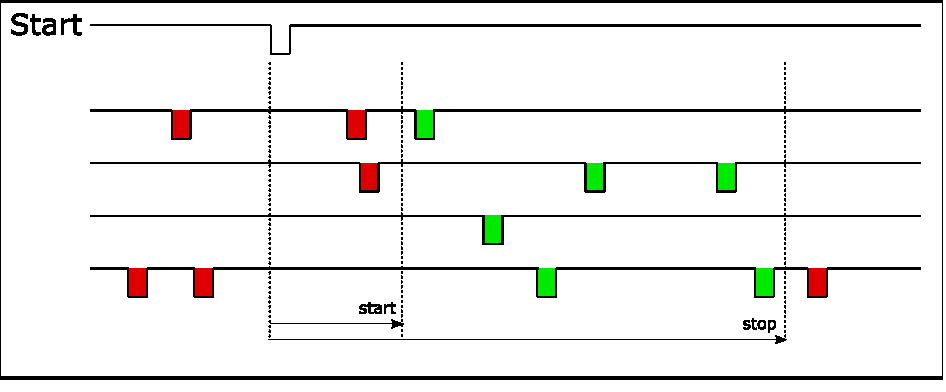
\includegraphics[width=0.7\textwidth]{figures/grouping.pdf}
        \caption{Acquired hits are merged to groups as explained in the
            text.\label{fig:grouping}}
    \end{center}
\end{figure*}
%
 
Figure~\ref{fig:grouping} shows a corresponding timing diagram. The user can
define the range of a group, i.e., the time window within which hits on the
stop channels are recorded. Hits occurring outside that time window are
discarded. 

\ifxHPTDC{
    The start and stop values for grouping can also be negative. This allows
    to configure the \deviceName\ for common-start, common-stop, or for groups
    that extend into both directions.

    The values are configured in \si{\pico\second}.
    \begin{align*}
        -2^{31} \le start \le stop \le 2^{31}-1
    \end{align*}
}{
     Different ranges can be set for each of the stop channels by setting
     corresponding values for \texttt{channel[i].start} and
     \texttt{channel[i].stop} values.

     The values need to be set as multiples of the bin size and must not be
     negative.
     \begin{align*}
        0 \le start \le stop \le 2^{16}-1
     \end{align*}

     If a second start is recorded within the range of a group, the current
     group is finished and a new group is started. Consecutive stops will
     be assigned to the new group (as long as they are within the group range).
}

 \ifxHPTDC{
    In single-board setups, it is recommended to also configure the gating
    blocks (see Page~\pageref{member:gating_block}) to similar parameters as
    the grouping functionality.
    This prevents data from being read out that is discarded by the grouping 
    code anyway. 
    Please note that the grouping parameters are given in \si{\pico\second}
    while the gating blocks are configured in cycles of the
    \SI{150}{\mega\hertz} clock. For more information on the gating 
    functionality, see Section~\ref{cp:gating}.
    
    In grouping mode, each call to \texttt{xHPTDC8\tu read\tu hits()} will
    return a group of timestamps relative to some trigger event.  At the
    beginning of each group, an additional hit with channel number 255 is
    returned. This hit contains the absolute time of the group.  The absolute
    time of the remaining hits can be obtained by adding this value to the
    relative time of each hit. Otherwise, the call returns all available
    timestamps as absolute timestamps counting upwards from \texttt{xHPTDC8\tu
    start\tu capture().}
}{}   
